% ---------------------------------------------------------------------------------------------
% DRAFT -- not part of the thesis. Proposed new section for Chapter 5 (Chapter5.tex), to go
% between \section{Dependence on noise level} and \section{Summary}.
%
% Sources: hubbletilus_noise_moves.ipynb and hubbletilus_noise_moves_0p05.ipynb (the full runs with
% tilts of +-0.1 and +-0.05 deg), thesis_drafts/noise_moves_analysis.py (linearized numbers, run
% residuals) and thesis_drafts/make_noise_moves_figure.py (the figure). To adopt it, copy
% thesis_drafts/figures/noise_moves.png to Masters_Thesis/figures/.
% ---------------------------------------------------------------------------------------------

\section{Observations after known moves of the secondary}\label{sec:noise_moves}

Section~\ref{sec:noise_de} showed that the Hubble DE estimate is limited by the observation noise, amplified along the decenter--tilt degeneracy. There are two ways to raise its precision: collect more light, which reduces every error as $1/\sqrt{M}$ for $M$ exposures, or make the observations themselves more informative. Phase diversity~\citep{Gonsalves1982} does the latter by recording a second image with a known added aberration, usually defocus. The alignment mechanism can provide the added aberration itself: the secondary is moved by known amounts relative to its unknown position, and the PSFs are recorded again at each position. This section asks how much such moves improve the Hubble estimate, first with the linearized analysis of Section~\ref{sec:noise_de} and then with full runs of the pipeline for two move sizes.

If the secondary is observed at $\boldsymbol{\theta}_{\mathrm{true}}+\boldsymbol{\delta}_m$, $m=0,\dots,M-1$, with $\boldsymbol{\delta}_0=\mathbf{0}$ and every $\boldsymbol{\delta}_m$ known, the DE objective (equation~\ref{eq:de_cost}) becomes a sum over positions,
\begin{equation}
S(\boldsymbol{\theta}) = \sum_{m=0}^{M-1}\sum_{f\in\mathcal{F}}\sum_{k=1}^{N_z}\left[c_{f,k}(\boldsymbol{\theta}+\boldsymbol{\delta}_m) - c_{m,f,k,\mathrm{obs}}\right]^2,
\label{eq:de_cost_moves}
\end{equation}
and equation~(\ref{eq:lscov}) becomes
\begin{equation}
\mathrm{Cov}(\hat{\boldsymbol{\theta}}) =
\Bigl(\sum_{m}\mathbf{J}_m^{\top}\mathbf{J}_m\Bigr)^{-1}
\Bigl(\sum_{m}\mathbf{J}_m^{\top}\mathbf{N}_{\mathrm{all}}\mathbf{J}_m\Bigr)
\Bigl(\sum_{m}\mathbf{J}_m^{\top}\mathbf{J}_m\Bigr)^{-1},
\label{eq:lscov_moves}
\end{equation}
where $\mathbf{J}_m$ is the Jacobian of the coefficients of all fields at $\boldsymbol{\theta}_{\mathrm{true}}+\boldsymbol{\delta}_m$ and $\mathbf{N}_{\mathrm{all}}$ is as before. If every $\boldsymbol{\delta}_m$ is zero, the $M$ exposures are repeats, all $\mathbf{J}_m$ are equal and every standard deviation falls by $\sqrt{M}$. The benefit of moving is therefore measured against the same number of exposures at the nominal position: we define the gain as the standard deviation from $M$ such exposures divided by the standard deviation with the moves.

\begin{figure*}
    \centering
    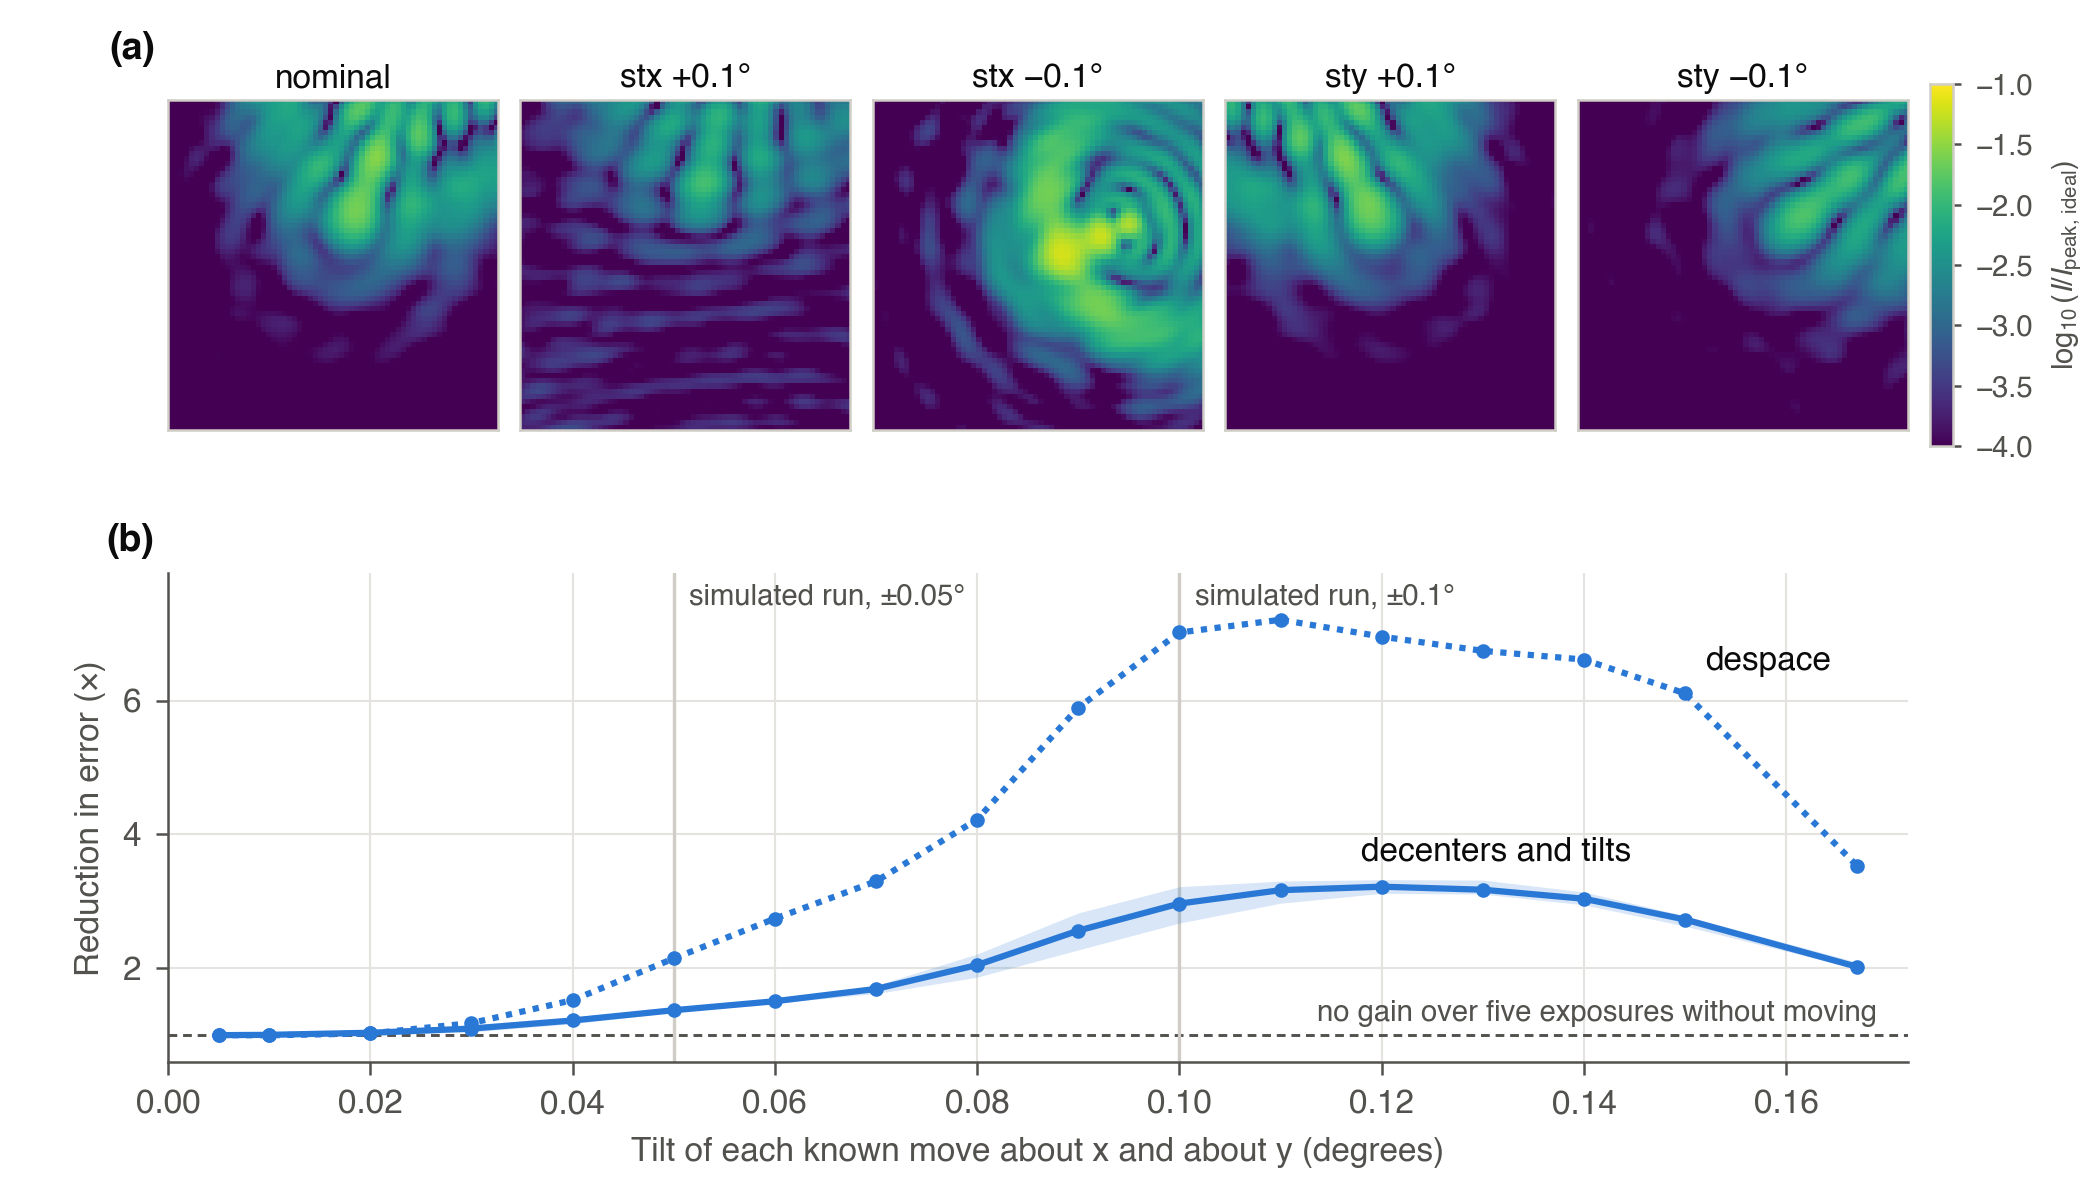
\includegraphics[width=\textwidth]{figures/noise_moves.png}
    \caption[Known moves of the Hubble secondary.]{Known moves of the Hubble secondary. (a) On-axis PSF, on a logarithmic scale relative to the ideal peak, at the injected misalignment and after the four known tilts of $\pm0.1$ degrees used in the first simulation. (b) Predicted reduction in the noise-limited error of the DE estimate relative to five exposures at the nominal position (equation~\ref{eq:lscov_moves}), for five positions: the nominal one and tilts of $\pm\Delta$ about $x$ and about $y$. The band spans the four decenter and tilt parameters and the solid line is their mean; the dotted line is the despace. The vertical lines mark the two simulated designs.}
    \label{fig:noise_moves}
\end{figure*}

Figure~\ref{fig:noise_moves}b shows the gain for designs of five positions: the nominal one and tilts of $\pm\Delta$ about $x$ and about $y$. Moves of $0.01$ degrees or less give no gain, and moves of $0.02$ degrees at most 7\%. The PSF responds almost linearly to such small changes, so a moved PSF carries nearly the same information as a repeated exposure, and the improvement is essentially the factor $\sqrt{5}$ from five times the exposure. The gain rises from about $0.03$ degrees, peaks near $0.11$--$0.12$ degrees at 3.1--3.3 on the decenters and tilts and 7.2 on the despace, and falls for larger moves, possibly because these push the PSF toward the edge of the $64\times64$-pixel cutout (Figure~\ref{fig:noise_moves}a). What matters is the amount of known coma a move adds rather than the actuator that makes it. In coma, one degree of secondary tilt is equivalent to about $10$\,mm of decenter, and decenter moves matched in coma give similar gains: 2.3--2.7 on the decenters and tilts for $\pm1$\,mm, but none for $\pm100$--$200\,\mu\mathrm{m}$. Moves in despace mainly improve the despace estimate (by $1.9$ for $\pm100\,\mu\mathrm{m}$, against at most $1.2$ for the other parameters), and moves of $\pm400\,\mu\mathrm{m}$ degrade every parameter.

To test the prediction, we repeated the Hubble benchmark of Chapter~\ref{chap:hubble} twice, keeping the injected misalignment: with the nominal position and tilts of $\pm0.1$ degrees about $x$ and about $y$, close to the predicted optimum, and with tilts of $\pm0.05$ degrees, for which the predicted gain from the moves is only 1.3--2.2. Each of the five positions was observed at the five fields of Section~\ref{sec:hubble} with independent noise ($\sigma=0.01$), giving 25 PSFs and 375 coefficients per run; the two runs share the same noise draws. The likelihood (equation~\ref{eq:loglike}) and the DE objective (equation~\ref{eq:de_cost_moves}) sum over the positions. Each moved position uses the calibration covariance $\boldsymbol{\Sigma}_f$ of its field; this is an approximation, but a $0.1$-degree move lies well within the distribution from which $\boldsymbol{\Sigma}_f$ was estimated. The noise realization differs from that of Chapter~\ref{chap:hubble}. Since an evaluation now needs 25 PSFs, the five positions were computed in parallel, which kept the time per evaluation close to that of the nominal run.

With tilts of $\pm0.1$ degrees, Nautilus needed $75\,400$ likelihood evaluations ($N_{\mathrm{eff}}\approx1.6\times10^4$). Unlike the nominal run, whose $sdx$ and $sdy$ marginals are nearly flat (Figure~\ref{fig:hubble_corner}), the posterior concentrates on a lattice of modes about $100\,\mu\mathrm{m}$ apart in $sdx$ and $sdy$, the highest of which contains the truth. The lattice comes from the prior transform, which rounds the tilts to $0.01$ degrees (Section~\ref{sec:prior_like}): a tilt step of $0.01$ degrees is compensated by about $100\,\mu\mathrm{m}$ of decenter, so each neighbouring tilt value produces its own mode. The weighted median of the final 100 posterior samples was $(53.17,\allowbreak\,-114.35,\allowbreak\,39.05,\allowbreak\,0.13,\allowbreak\,-0.04)$, within $1\,\mu\mathrm{m}$ of the truth on both decenters, compared with $113\,\mu\mathrm{m}$ on $sdy$ in the nominal run. Its on-axis WFE, $1.9\times10^{-3}$ waves, is already close to the final result of the nominal run. Because the tilt posterior is narrower than the rounding step, nearly all of the weight of the final 100 samples lies on the true tilt values, and the 2.1\%--97.9\% DE bounds on $stx$ and $sty$ collapse to single values. SciPy holds a parameter with equal bounds fixed, so we widened each collapsed bound by one rounding step on each side, to $(0.12,\,0.14)$ and $(-0.05,\,-0.03)$ degrees.

With tilts of $\pm0.05$ degrees, Nautilus needed $60\,900$ evaluations ($N_{\mathrm{eff}}\approx1.4\times10^4$). The posterior shows the same lattice of modes, but the modes carry similar weight, and most of the weight of each tilt is spread over three grid values, $0.11$--$0.13$ and $-0.05$ to $-0.03$ degrees. No bound collapsed, and the DE bounds on the decenters stayed wide, $220\,\mu\mathrm{m}$ on $sdx$ and $125\,\mu\mathrm{m}$ on $sdy$ (against 327 and $378\,\mu\mathrm{m}$ in the nominal run). The weighted median of the final 100 samples, $(51.05,\allowbreak\,-111.11,\allowbreak\,39.15,\allowbreak\,0.13,\allowbreak\,-0.04)$, was still within $3\,\mu\mathrm{m}$ of the truth on both decenters, with an on-axis WFE of $5.2\times10^{-3}$ waves.

In both runs DE used deferred updating, as in the TMA run, so that each generation could be evaluated in parallel. In the $\pm0.1$-degree run, its cost came within 1\% of its final value by generation 47, and the run was stopped by hand after 137 generations at $S=2.78\times10^{-4}$. The expected minimum of the five-position objective is $(2.84\pm0.23)\times10^{-4}$, so the run reached the noise floor; L-BFGS-B polishing left the solution unchanged. Table~\ref{tab:noise_moves} compares the residuals with the predicted standard deviations. For this run, every residual lies within 0.9 standard deviations of zero, and the squared Mahalanobis distance of the residual vector is 2.9, a typical value for five degrees of freedom. The predicted standard deviations are 6.0--7.2 times smaller than for the nominal position alone on the decenters and tilts and 16 times smaller on the despace. Of these factors, $\sqrt{5}\approx2.2$ comes from the additional exposures and 2.7--3.2 (7.0 on the despace) from the moves. Image quality improves accordingly. Propagating the covariance to the on-axis OPD by Monte Carlo (300 draws) gives a median RMS WFE of $1.5\times10^{-4}$ waves (16th--84th percentiles $0.8$--$2.4\times10^{-4}$), against $1.2\times10^{-3}$ waves for the nominal position. The run reached $2.1\times10^{-4}$ waves, compared with $1.35\times10^{-3}$ waves in Chapter~\ref{chap:hubble}.

The $\pm0.05$-degree run was given its full 1000 generations. Its cost came within 1\% of its final value by generation 48 and within 0.1\% by generation 70, ending at $2.75\times10^{-4}$ against an expected $(2.83\pm0.23)\times10^{-4}$; polishing moved the estimate by less than $10^{-7}$. Its residuals lie between 1.0 and 1.7 standard deviations from zero, larger than in the $\pm0.1$-degree run but consistent with the noise. They come in pairs along the two degenerate directions, $sdy$ with $stx$ ($z=-1.54$ and $+1.54$) and $sdx$ with $sty$ ($z=-1.70$ and $-1.63$), and the squared Mahalanobis distance of the residual vector, 5.4, is again typical for five degrees of freedom. The predicted standard deviations are 3.0--3.1 times smaller than for the nominal position alone on the decenters and tilts and 4.8 times smaller on the despace. Of these factors, $\sqrt{5}$ comes from the additional exposures and only 1.3--1.4 (2.2 on the despace) from the moves, as Figure~\ref{fig:noise_moves}b predicts. The predicted median on-axis WFE is $2.9\times10^{-4}$ waves (16th--84th percentiles $1.6$--$4.3\times10^{-4}$), and the run reached $1.95\times10^{-4}$ waves.

\begin{table}
\centering
\small
\setlength{\tabcolsep}{4pt}
\caption[Noise-limited precision with known moves of the Hubble secondary.]{Noise-limited precision of the Hubble DE estimate from the nominal position alone (Table~\ref{tab:noise_params}) and from the nominal position with tilts of $\pm0.05$ or $\pm0.1$ degrees about $x$ and about $y$ (predicted s.d., equation~\ref{eq:lscov_moves}), with the residuals $\boldsymbol{\theta}_{\mathrm{true}}-\mathbf{c}$ of the two five-position runs; $z$ is the ratio of each residual to the predicted standard deviation of its run. Translations are in $\mu$m and tilts in degrees.}
\label{tab:noise_moves}
\begin{tabular}{llllllll}
\hline
 & \textbf{Nominal} & \multicolumn{3}{c}{\textbf{Tilts of $\boldsymbol{\pm0.05^{\circ}}$}} & \multicolumn{3}{c}{\textbf{Tilts of $\boldsymbol{\pm0.1^{\circ}}$}} \\
\textbf{Parameter} & \textbf{s.d.} & \textbf{s.d.} & \textbf{Residual} & $\boldsymbol{z}$ & \textbf{s.d.} & \textbf{Residual} & $\boldsymbol{z}$ \\
\hline
sdx & $3.62$ & $1.21$ & $-2.05$ & $-1.70$ & $0.61$ & $0.16$ & $0.26$ \\
sdy & $3.96$ & $1.29$ & $-1.99$ & $-1.54$ & $0.56$ & $-0.006$ & $-0.01$ \\
sdz & $0.075$ & $0.016$ & $-0.015$ & $-0.97$ & $0.0048$ & $-0.0043$ & $-0.90$ \\
stx & $3.8\times10^{-4}$ & $1.2\times10^{-4}$ & $1.9\times10^{-4}$ & $1.54$ & $5.3\times10^{-5}$ & $9.9\times10^{-6}$ & $0.19$ \\
sty & $3.6\times10^{-4}$ & $1.2\times10^{-4}$ & $-1.9\times10^{-4}$ & $-1.63$ & $5.7\times10^{-5}$ & $2.2\times10^{-5}$ & $0.39$ \\
\hline
\end{tabular}
\end{table}

The moves do not break the decenter--tilt degeneracy. The correlations between the decenters and the perpendicular tilts are $r=-0.989$ for $sdy$--$stx$ and $r=+0.995$ for $sdx$--$sty$ with tilts of $\pm0.1$ degrees, and $-0.997$ and $+0.996$ with tilts of $\pm0.05$ degrees, against $-0.996$ and $+0.995$ for the nominal position; the standard deviations of the four decenters and tilts shrink by similar factors. The gain comes instead from sensitivity. The known coma added by each move makes the coefficients respond more strongly to every parameter, much as the known defocus of phase diversity does. Separating a decenter from the compensating tilt would still require observables that distinguish the two motions (Section~\ref{sec:conc_future}). The two runs also show how little the degenerate directions matter for the image. The decenter errors of the $\pm0.05$-degree run, about $2\,\mu\mathrm{m}$, are more than ten times those of the $\pm0.1$-degree run, yet its on-axis WFE is no larger ($1.95$ against $2.1\times10^{-4}$ waves), because an error along a degenerate direction barely changes the on-axis wavefront.

The gain also depends on knowing the moves. In the linearized model, an unknown error $\boldsymbol{\epsilon}_m$ in move $m$ shifts the estimate by $\bigl(\sum_{k}\mathbf{J}_k^{\top}\mathbf{J}_k\bigr)^{-1}\mathbf{J}_m^{\top}\mathbf{J}_m\boldsymbol{\epsilon}_m$. For the $\pm0.1$-degree design, such errors become as large as the noise term once they reach about $0.8\,\mu\mathrm{m}$ in decenter, $5\times10^{-5}$ degrees in tilt or $5$\,nm in despace per move. Less accurately known moves would have to be estimated as additional parameters, which would give up part of the gain. The analysis assumes that the moved positions stay within the range where $\boldsymbol{\Sigma}_f$ and the forward model apply, and it treats additive noise only (Section~\ref{sec:noise_model}). The two full runs share one noise realization and one injected misalignment, and the most useful move size depends on the misalignment, since a move must be comparable to the coma already present to change the PSF appreciably.

% ---------------------------------------------------------------------------------------------
% SUGGESTED FOLLOW-ON EDITS (not applied; the thesis is unchanged)
%
% Chapter5.tex, opening paragraph -- replace
%   "It then asks how the results change with the noise level (Section~\ref{sec:noise_sweep})."
% with
%   "It then asks how the results change with the noise level (Section~\ref{sec:noise_sweep}) and
%    how much observations after known moves of the secondary improve the precision
%    (Section~\ref{sec:noise_moves})."
%
% Chapter5.tex, Summary -- after "... is therefore a natural route to higher precision." add
%   "Observing the Hubble secondary after four known tilts of $\pm0.1$ degrees does not reduce the
%    degeneracy but makes the coefficients more sensitive to the alignment: the predicted errors
%    fall 2.7--3.2 times more than with five exposures at the nominal position on the decenters
%    and tilts, and 7.0 times more on the despace. A full run of the pipeline with these moves
%    recovered both decenters to within $0.2\,\mu\mathrm{m}$, with an on-axis WFE of
%    $2.1\times10^{-4}$ waves. Tilts of $\pm0.05$ degrees gave less than half of this gain, as
%    predicted."
%
% Chapter6.tex, "Breaking the degeneracies" -- after the sentence citing phase-diverse images add
%   "Section~\ref{sec:noise_moves} tested a variant in which the secondary itself supplies the
%    diversity: known tilts of $\pm0.1$ degrees reduced the Hubble errors by a further factor of
%    about three, through sensitivity rather than by breaking the degeneracy."
%
% Chapter 1 (contributions) and the abstract could mention the result in one clause, e.g.
%   "... and shows that observations after known moves of the secondary reduce these errors
%    severalfold."
% ---------------------------------------------------------------------------------------------
